\chapter{API Design}

We created an API that contains the whole game logic, so it would be easy to exchange it with a game logic someone else may want. The API can be seen in the \href{https://github.com/kerko/epic/tree/master/project/src/nl/fontys/epic/core}{epic.core} package or in the following class diagram. 
%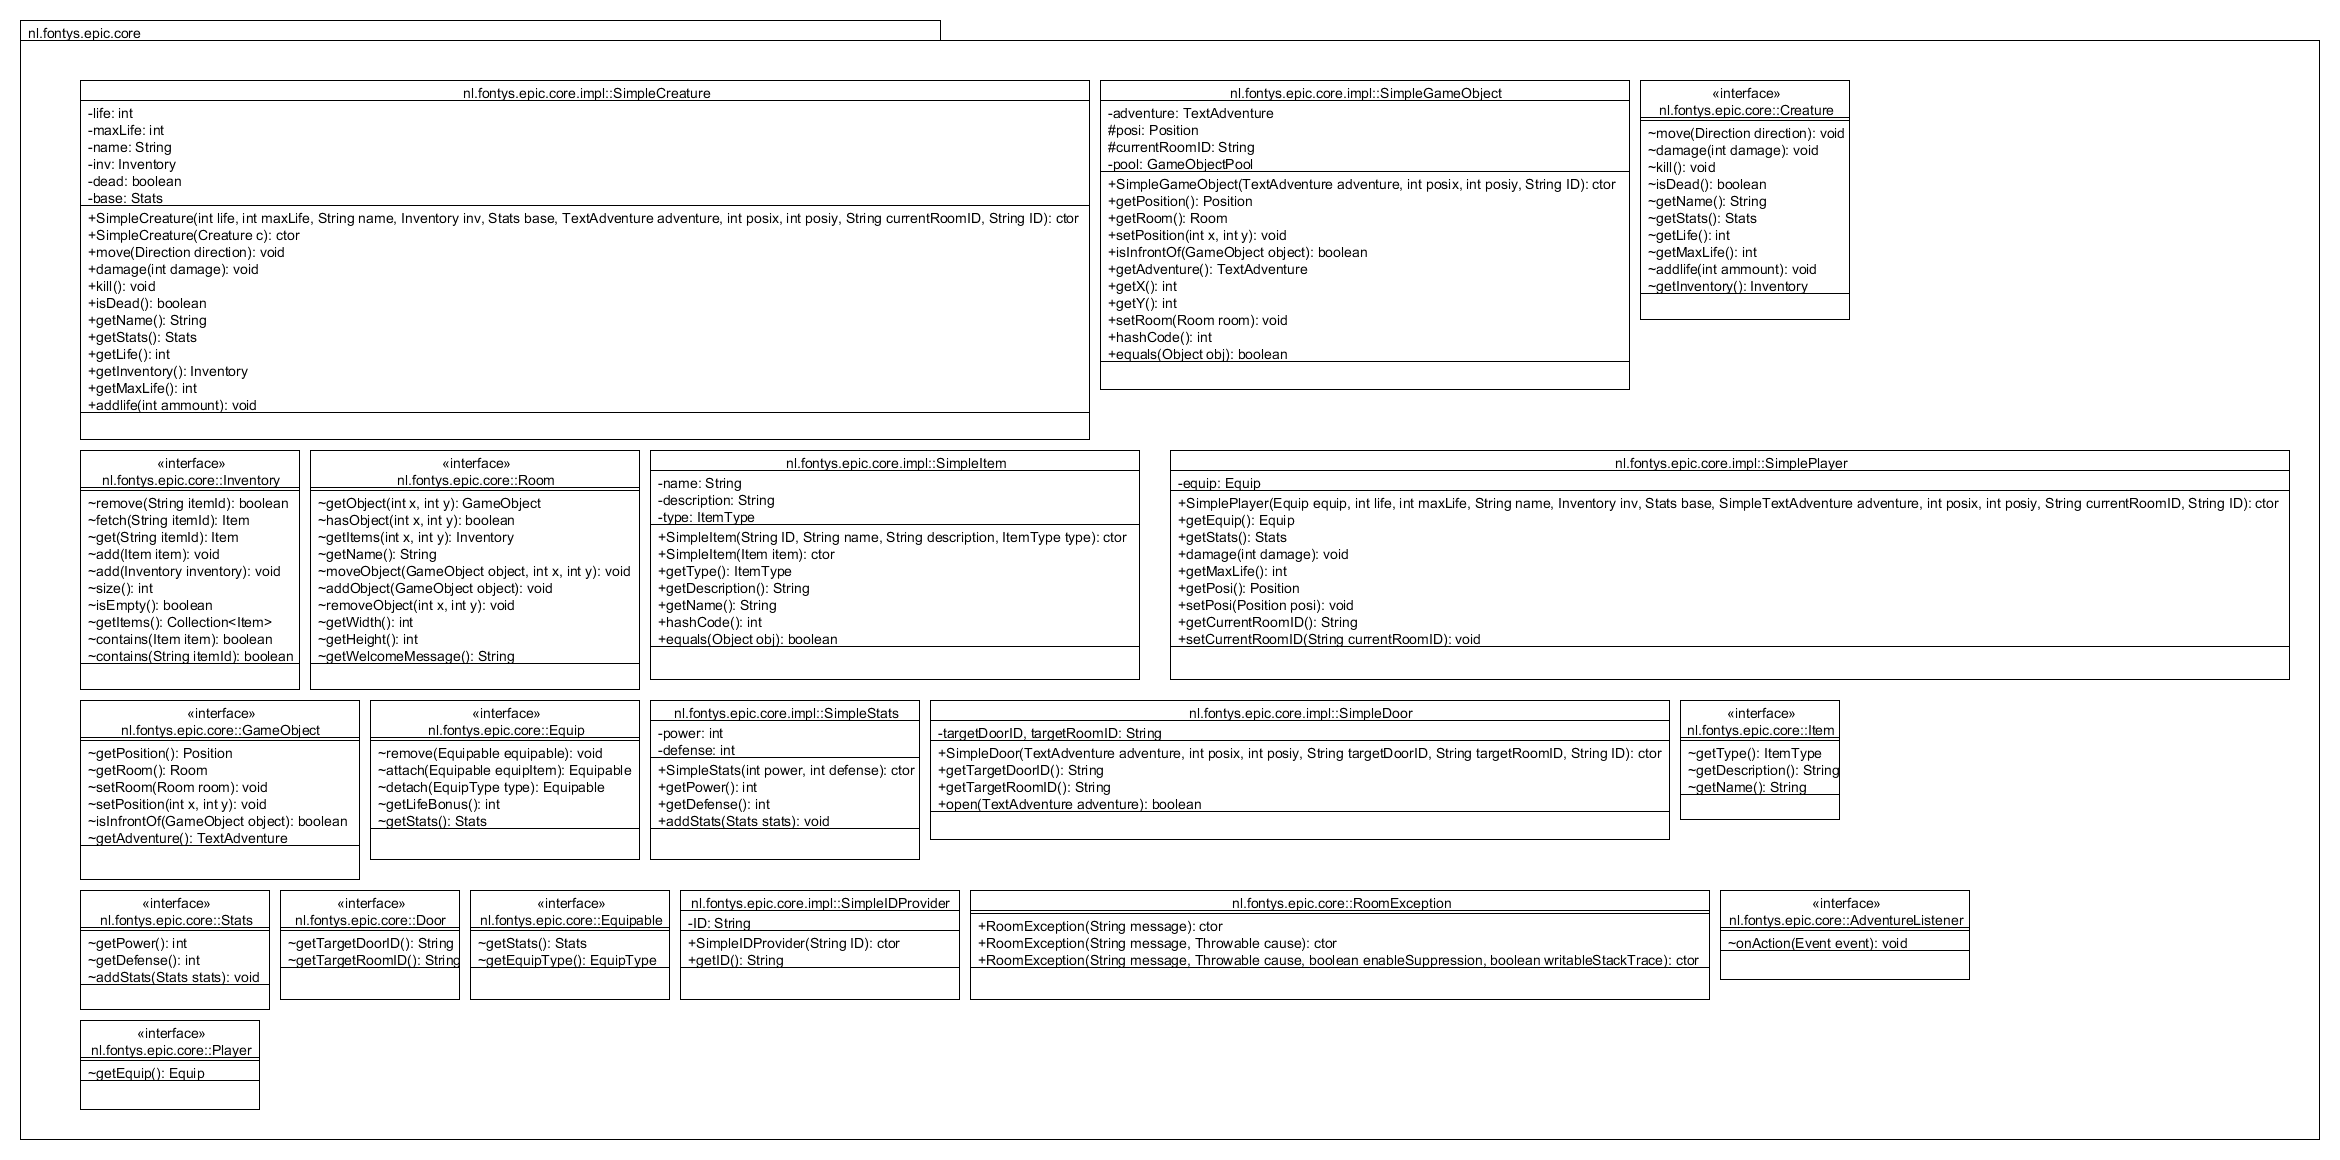
\includegraphics{assest/package-core.png}

Our api consists of theses entities : 
\begin{itemize}
\item Room
\item Door
\item Item
\item Equip
\item Inventory
\item Player
\end{itemize}
All entities provide basic functionalities which belong to the game, like items offering stats and the inventory is capable of keeping items. For a complete overview of all the functions see the java doc.

And the utility classes, including enums, for the types of items and equip:
\begin{itemize}
\item GameObject - Superclass of alle GameObjects 
\item IDProvider - Superclass of everything to supply ID's.
\item Stats -Helper class to manage the different stats on a item or creature.
\item RoomException - Gets fired at different times, related to issues with the room, like no valid room link on doors.
\item AdventureListener
\item EquipType - Enum for the slots of equip a player can carry.
\item ItemType -  Enum for the different types of items.
\end{itemize}


We provided a simple sample implementation of the API for anyone to use or build upon, which can be found in \href{https://github.com/kerko/epic/tree/master/project/src/nl/fontys/epic/core/impl}{epic.core.impl}


